%%%%%%%%%%%%%%%%%%%%%%%%%%%%%%%%%%%%%%%%%%%%%%%%%%%%%%%%
%GRASS PROMOTION FLYER                                 %
%(c) 2007 GRASS PROMOTION TEAM                         %
%    Translation: Milena Nowotarska                    %
%GNU Free Documentation License                        %
%Version 1.2                                           %
%Needs leaflet.cls				       %
%www.ctan.org/tex-archive/macros/latex/contrib/leaflet/%
%%%%%%%%%%%%%%%%%%%%%%%%%%%%%%%%%%%%%%%%%%%%%%%%%%%%%%%%

%Sometimes printing engines need the 2nd side upside down
%in this case, use tumble (which is default) instead of notumble
%If this causes problems, use notumble
%If you need a foldmark, delete nofoldmark
\documentclass[notumble,a4paper,10pt,nofoldmark]{leaflet}
\usepackage{helvet,courier,xcolor}

% Set Helvetica as the default font
\renewcommand*\familydefault\sfdefault
% Let LaTeX knows that pictures are found in ./pix
\graphicspath{{pix/}}

% Setting up things for the captions
\usepackage{caption}[2004/07/16]
\captionsetup{%
  font={small,it},%
  labelformat=empty,% Leaves out label: ``Figure 1''
  labelsep=none,%
  aboveskip=0pt%
}
% Defining a new 'figure' environment for the document
\newenvironment{myfig}[1][0pt plus 1.5ex minus .5ex]{\par\vspace*{#1}\begin{minipage}{\textwidth}\centering}{\end{minipage}}

% Defining the GRASS homepage
\newcommand{\GRASSurl}{\url{http://grass.osgeo.org}}

% Define a color for the URIs
\definecolor{darkblue}{RGB}{0,0,88}

\usepackage{hyperref}
% Setting up some document info
\hypersetup{%
  colorlinks=true,%
  urlcolor=darkblue,% Redefine this color to change URIs color
  pdfauthor={The GRASS Community},%
  pdftitle={GRASS GIS: Efektywność dzięki Wolności \& Przejrzystości},%
  pdfsubject={Ulotka promocyjna GRASS},%
  breaklinks=true,%
  plainpages=false%
}

% Title page stuff
\title{\textbf{\huge GRASS GIS}\\%
\textsl{Efektywność dzięki Wolności \& Przejrzystości}}
\author{Społeczność GRASS-a}
\date{
\includegraphics[width=\textwidth]{pix/grasslogo_vector}\\[2ex]
\large\GRASSurl}

\begin{document}

\maketitle
\thispagestyle{empty}% Necessary to leave out the page number on the first page

\newpage

\section{Co to jest GRASS}

GRASS (Geographic Resources Analysis Support System) is a free and Open Source Software for performing spatial analysis. Składa się z ponad 350 modułów do przetwarzania danych wektorowych (2D/3D), rastrowych i voxel. Many interfaces to other programs in related domains like geostatistics, databases, mapserver and even other GIS software exist. It is the largest Open Source GIS. It can serve as a Desktop GIS and as the backbone of a complete GIS Infrastructure.

\section{Gdzie używa się GRASS-a}

GRASS jest używany na całym śwecie przez środowiska akademickie, komercyjne jak i przez władze publiczne. GRASS wykazał się dużym potencjałem do rozwiązywania problemów geoprzestrzennych w wielu zastosowaniach na  świecie.

\section{Historia}

GRASS was originally developed in the beginning of the 1980's by the US Army Construction Engineering Research Laboratories (USA-CERL) and was published as public domain software. When the USA-CERL withdrew from GRASS development, an international developer team took over this work. Since 1999, GRASS has been published as free software under the terms of the GNU General Public Licence.
\begin{myfig}[1.5ex]
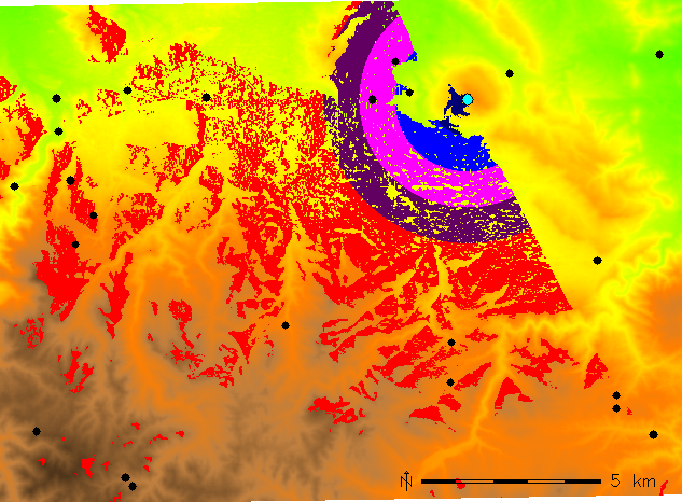
\includegraphics[width=0.7\textwidth]{pix/visibility}
\captionof{figure}{Viewshed analysis performed with GRASS}
\end{myfig}

\section{Filozofia Open Source}

The Open Source philosophy provides the user the ability to see the source code and structure of the program which offers a great transparency. Users can extend the program for their own needs. Immediate source code peer review increases the quality. With the help of the extension manager new modules can be created without GRASS package source code.

\section{Technical Data Sheet}

\subsection{Licencja}

GNU General Public License (Free Software Foundation)

\subsection{Supported platformy}

GRASS działa na prawie wszystkich platformach operacyjnych. Zarówno na GNU/Linux, zgodnych z POSIX systemach Unix, jak i MS Windows oraz MacOS X.

\subsection{Konstrukcja}

\begin{itemize}
\item Modły
\item Składa się z ponad 350 modułów
\end{itemize}

\subsection{Języki programowania}

\begin{itemize}
\item ANSI C
\item Interfejs GRASS- SWIG
\item Python dla aplikacji WebGIS
\item Wersja dla Javy: JGRASS
\end{itemize}

\subsection{Możliwości zarządzania danymi}

\begin{itemize}
\item Przetwarzanie danych rastrowych / wektorowych / voxel
\item Modelowanie danych 2D / 3D rastrowych / wektorowych 
\item Opracowywanie zobrazowań
\item Topologia wektorowa / analizy sieciowe
\item Geostatystyki (interfejs dla R)
\end{itemize}

\begin{myfig}[1ex]
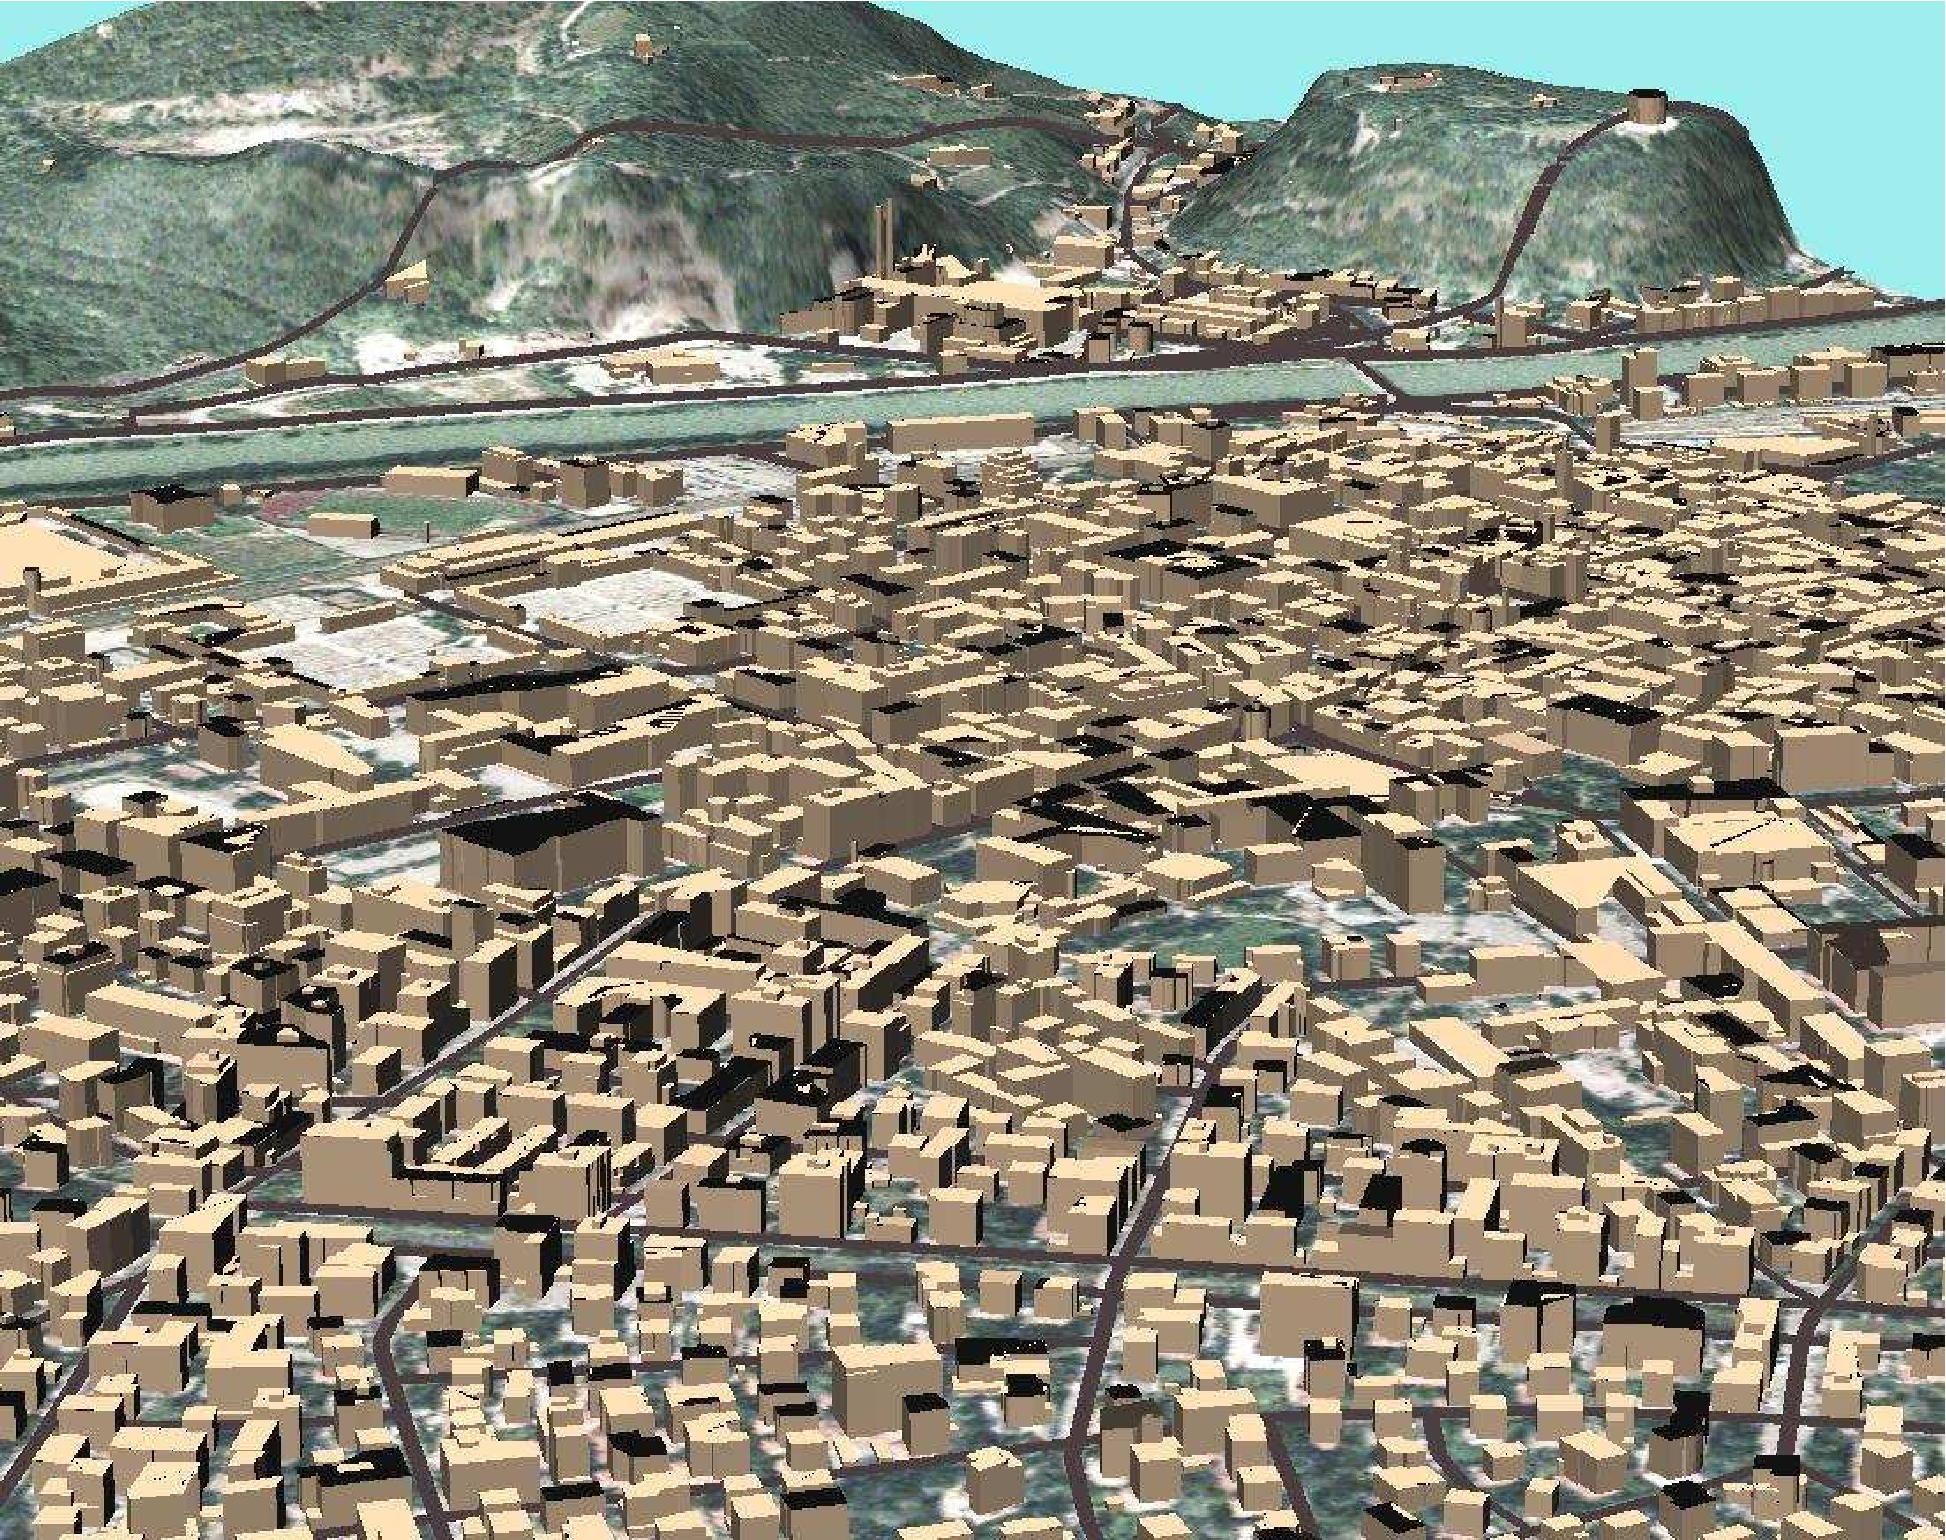
\includegraphics[width=0.7\textwidth]{pix/trento3d}
\captionof{figure}{Przelot nad Trydentem, Włochy}
\end{myfig}

\section{Obsługiwane formaty danych}

GRASS obsługuje prawie wszystkie popularne formaty danych gisowskich poprzez bibliotekę GDAL/OGR. Dodatkowo obsługuje także Open GIS Consortium's Simple Features.

\subsection{Formaty wektorowe}
ASCII, ARC/INFO ungenerate, ARC/INFO E00, Arc\-View SHAPE, BIL, DLG (U.S.), DXF, DXF3D, GMT, GPS-ASCII USGS-DEM, IDRISI, MOSS, MapInfo MIF, PostGIS, TIGER, VRML, \dots

\subsection{Formaty rastrowe}
ASCII, ARC/GRID, E00, GIF, GMT, TIF, PNG, Vis5D, SURFER (.grd),\dots
\begin{myfig}
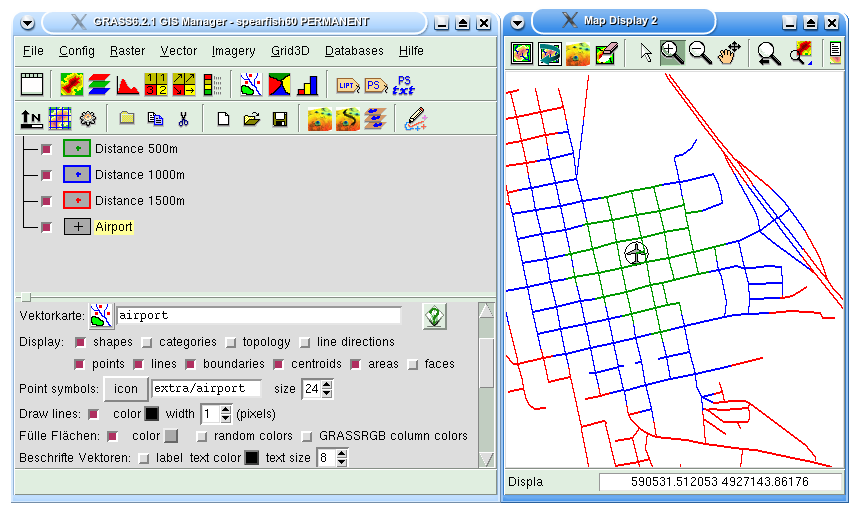
\includegraphics[width=0.7\textwidth]{pix/isodist}
\captionof{figure}{Domyślna konfiguracja GUI przedstawiająca możliwości analiz sieciowych GRASS-a}
\end{myfig}

\subsection{Formaty zobrazowań}

CEOS (SAR, SRTM, LANDSAT7 etc.), ERDAS LAN / IMG, HDF, LANDSAT TM/MSS, NHAP aerial photos, SAR, SPOT, \dots
\begin{myfig}[1.5ex]
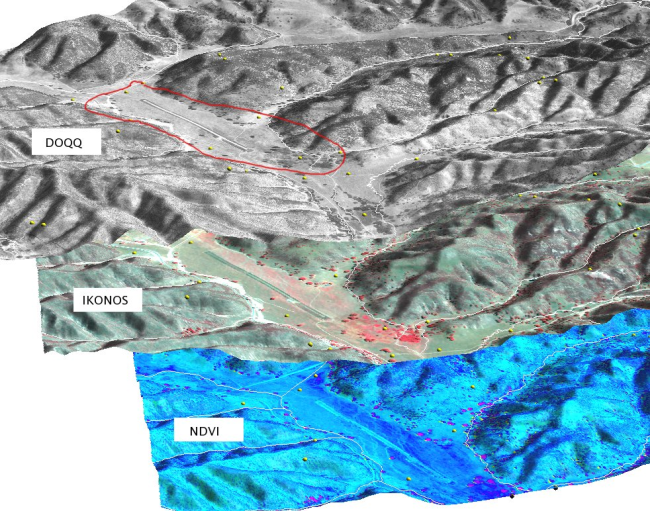
\includegraphics[width=0.7\textwidth]{pix/ndvi}
\captionof{figure}{Możliwości obróbki zobrazowań w GRASS-ie}
\end{myfig}

\subsection{Obsługa baz danych}

\begin{itemize}
\item PostgreSQL / PostGIS
\item MySQL
\item SQLite
\item ODBC
\item DBF
\end{itemize}

\subsection{Output}

\begin{itemize}
\item Moduły do produkcji map
\item NVIZ do wizualizacji danych 2.5D oraz 3D (tworzenie animacji \& przelotów)
%\item{GMT export}
%item{VRML}
\item VTK, POVray
\item WebGIS z użyciem Mapservera, Pythona, etc.
\end{itemize}

\subsection{Interoperacyjność z innymi programami GIS}

\begin{itemize}
\item Quantum GIS (Darmowa przeglądarka geodanych i nie tylko)
\item R- Language (Statystyki)
\item Gstat (Geostatystyki)
\item UMN Mapserver (Webmapping)
\end{itemize}

\section{Gdzie znaleźć więcej informacji}

\begin{itemize}
%\begin{flushleft}
\item{Strony internetowe projektu: \\\GRASSurl}
\item{GRASS Wiki: \\\url{http://grass.osgeo.org/wiki}}
\item{Zespół promocji GRASS-a: \\\url{malte@perlomat.de}}
\item{Listy mailingowe GRASS-a: \\\url{http://grass.osgeo.org/community/support.php}}
%\end{flushleft}
\item{Polskie forum GRASS-a: \\\url{http://forum.grass-gis.pl/}}
\item{Strony GRASS Polska: \\\url{http://www.grass-gis.pl/}}
\end{itemize}

\vfill
\section{OSGeo}

GRASS is a founding project of the Open Source Geospatial Foundation which has the aim to create high quality open source geospatial software. For further information visit the OSGeo homepage:
\begin{center}

\includegraphics[width=0.8\textwidth]{pix/OSGeo_CMYK}\\
\url{http://www.osgeo.org}
\end{center}

\end{document}
